\subsection{Изготовление и сборка.}

Все детали были изготовлены на 3д принтере. Изначально коробка была сделана без ребер жесткости, из-за чего при печати она деформировалась. Поэтому мы изменили конструкцию коробки, добавив ребра жесткости. 
\par\medskip

\begin{figure}[H]
	\centering
	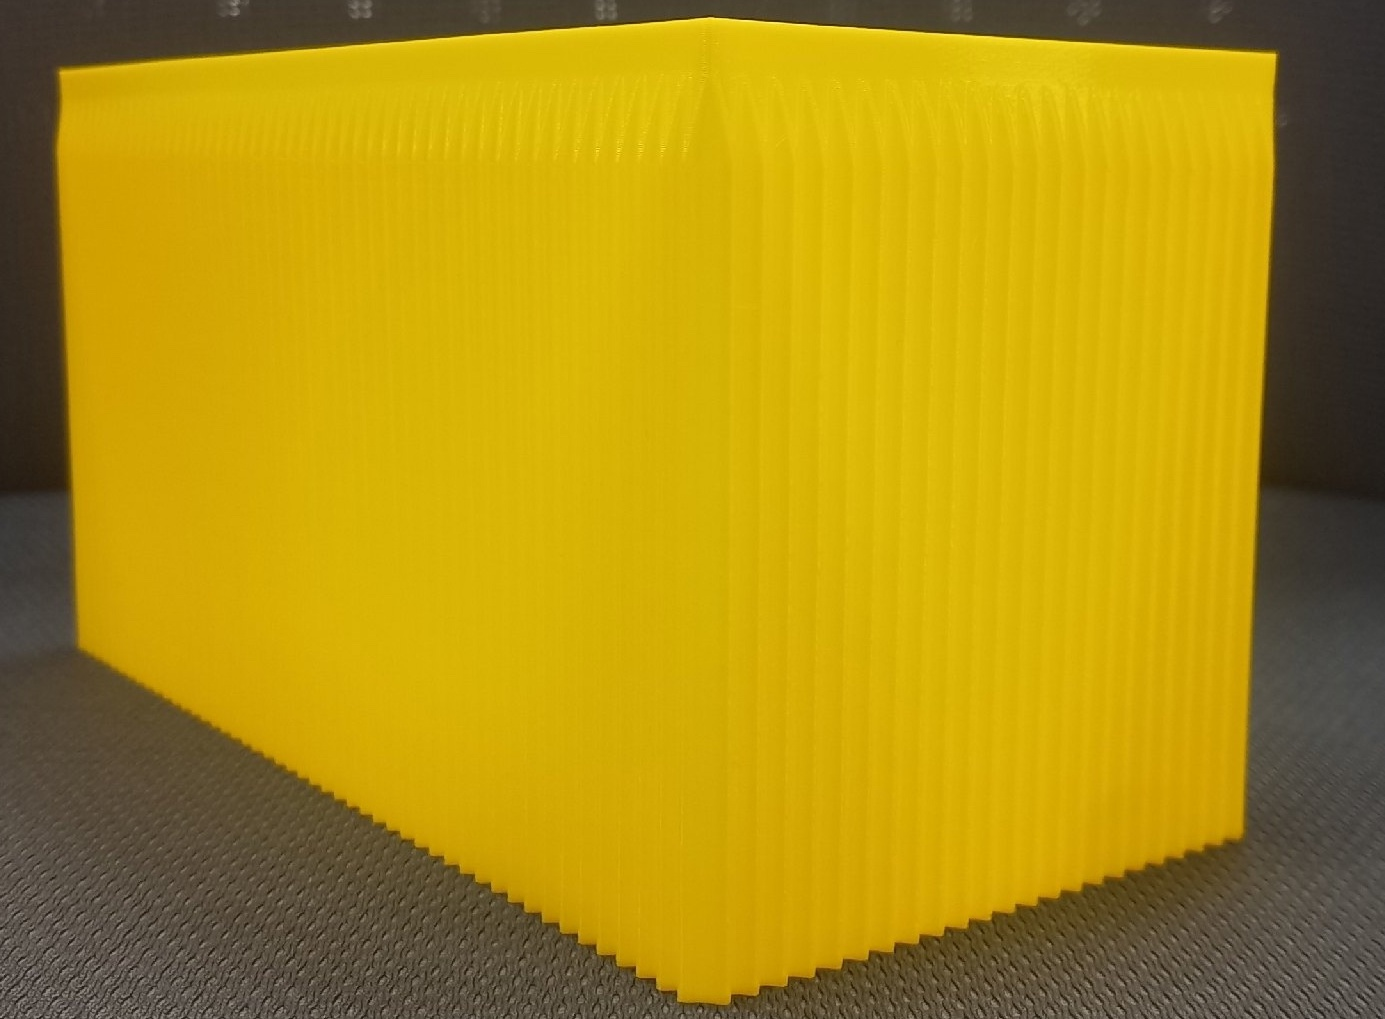
\includegraphics[width=12cm]{pics/korob.jpg}
	\caption{Короб для монет}
	\label{ris:korob_done}
\end{figure}

Электрическая схема была собрана из: шагового мотора, платы-драйвера шагового мотора, Arduino Nano, фототранзистора, ИК-светодиода, LCD экрана формата 2004 вместе с платой I2C, 2-х кнопок и провода USB (для питания). Схема соединений приведена ниже на рисунке~\ref{ris:scheme_electric}.

\begin{figure}[H]
	\centering
	\includegraphics[width=12cm]{pics/scheme_png.png}
	\caption{Схема соединения проводов}
	\label{ris:scheme_electric}
\end{figure}

При сборке были исправлены выявленные ошибки моделирования. В основном это касается отсутствующего отверстия для щели под ИК-светодиод и фототранзистор.
\par\medskip